\section{problem 4}
This problem will be conducted using python

\begin{lstlisting}
import numpy as np
import matplotlib.pyplot as plt
from scipy.signal import decimate, resample_poly
% load sample in and make a sample axis
x = np.loadtxt("SampleRateData.dat")
n = np.arange(len(x))
%downsample by 2, using decimate, since its decimation apply a fir filter,
M = 2
y = decimate(x, M, ftype='fir', zero_phase = True)
ny = np.arange(len(y))
%upsample by 2, using resample_poly, with an upfactor of 2 and a downfactor of 1
L = 2
z_up = np.zeros(len(y) * L)
z = resample_poly(y,up=L, down=1)
nz = np.arange(len(z))

%for ease of readability, plotting functionality has been omitted.
\end{lstlisting}

\begin{figure}[h]
    \centering
    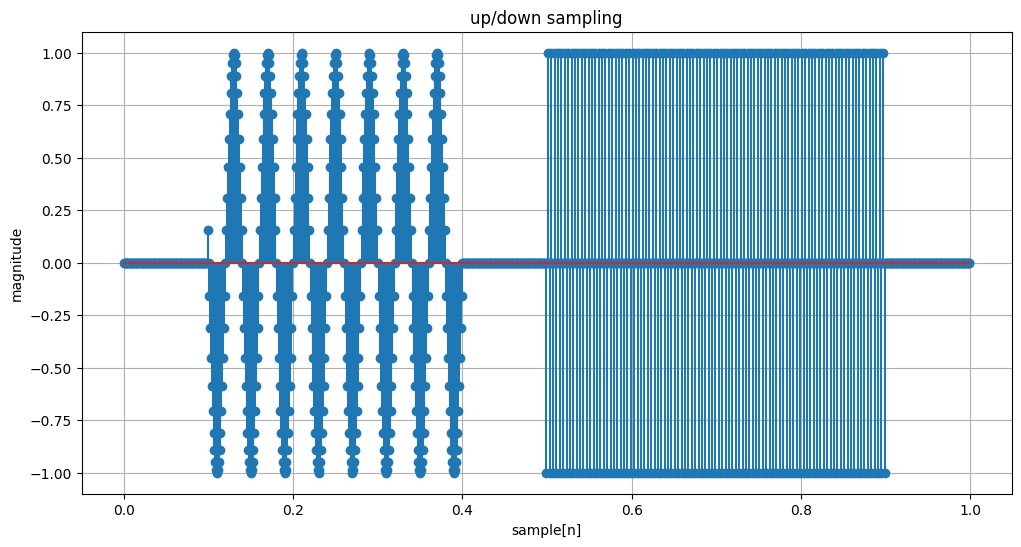
\includegraphics[width=0.7\linewidth]{p4_sample_load.png}
    
    \vspace{2mm}
    
    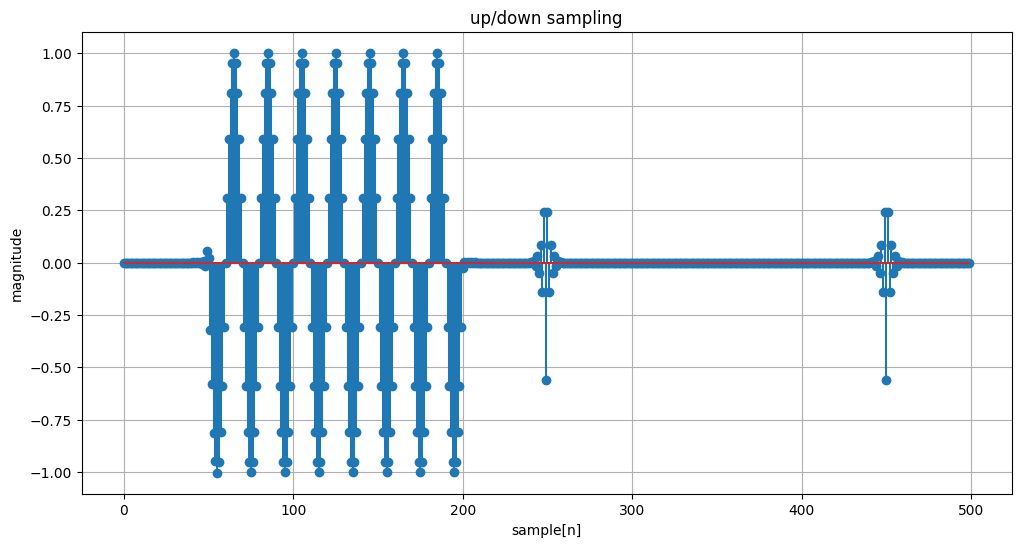
\includegraphics[width=0.7\linewidth]{p4_decimation.png}
    
    \vspace{2mm}
    
    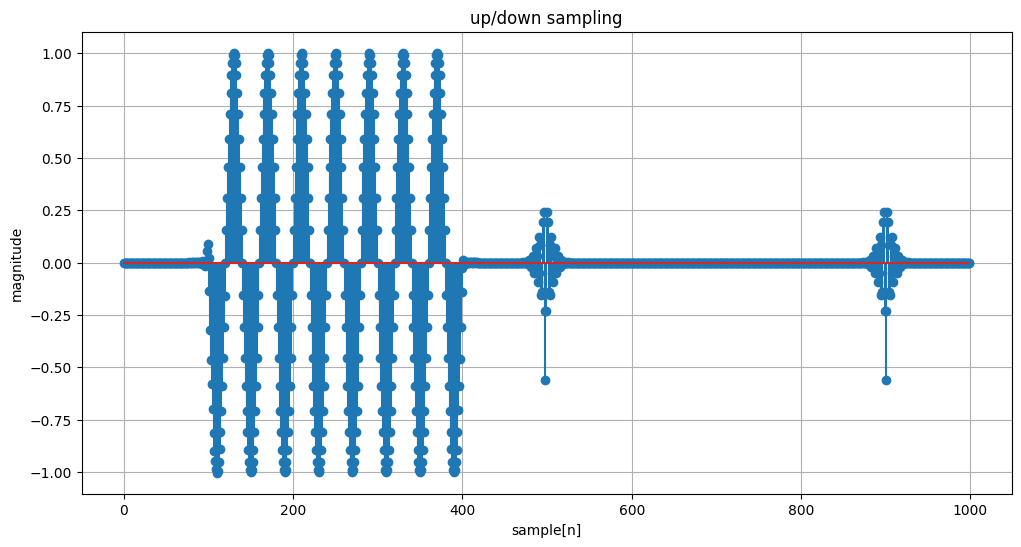
\includegraphics[width=0.7\linewidth]{p4_upsampling.png}
    
    \caption{top picture is the samples loaded into python, with no processing. The middle is after decimation,
    note that there are small changes the signal, that is because the decimation by a factor of two, bought with it a low pass filter,
    as the values suddely change, the filter has to react, however it cannot do so instantly. The last graph 
    is an interpolation by 2. It reconstructs, by estimation, some
    of the data lost to the decimation, however this is approximated, as it can never be recovered exactly.}
\end{figure}